
%%%%%%%%%%%%%%%%%%%%%%%%%%%%%%%%%%%%%%%%%%%%%%%%%%%%%%%%%%%%%%%%%%%%%%
%%%%                   Outcome
%%%%%%%%%%%%%%%%%%%%%%%%%%%%%%%%%%%%%%%%%%%%%%%%%%%%%%%%%%%%%%%%%%%%%%
%\color{blue}
\subsubsection{Glyph: \glyph{Outcome}}\label{sec:outcome}

In \ERs, an \glyph{outcome} represents the actualisation of a \glyph{statement} (\sect{statements}). For instance, if an \glyph{interaction} represents a non-covalent binding, the \glyph{outcome} represents the complex. If an \glyph{interaction} represents a genetic interaction, for instance derived from genetic screenings, the \glyph{outcome} represents the result of the presence of the two polymorphisms. If an \glyph{assignment} represents the phosphorylation of a protein, the \glyph{outcome} represents the phosphorylated form of this protein.

An \glyph{outcome} represent a particular instance of a realisation, and therefore, from one outcome must depart only one influence. An outcome being an \glyph{entity node}, it cannot receive influences. It exists. It cannot more or less exist. 

\begin{glyphDescription}

\glyphSboTerm SBO:0000409 ! interaction outcome

\glyphContainer  An \glyph{outcome} is represented by a black dot located on the arc of a \glyph{statement} (\sect{statements}). The diameter of the dot has to be larger than the thickness of the arc.

\glyphLabel An \glyph{outcome} has no identity on its own and does not carry any label. 

\glyphAux An \glyph{outcome} does not carry any auxiliary items.

\end{glyphDescription}

\begin{figure}[H]
  \centering
  \includegraphics[scale = 0.5]{images/outcome}
  \caption{The \ER glyph for \glyph{outcome}.}
  \label{fig:outcome}
\end{figure}

\begin{figure}[H]
  \centering
  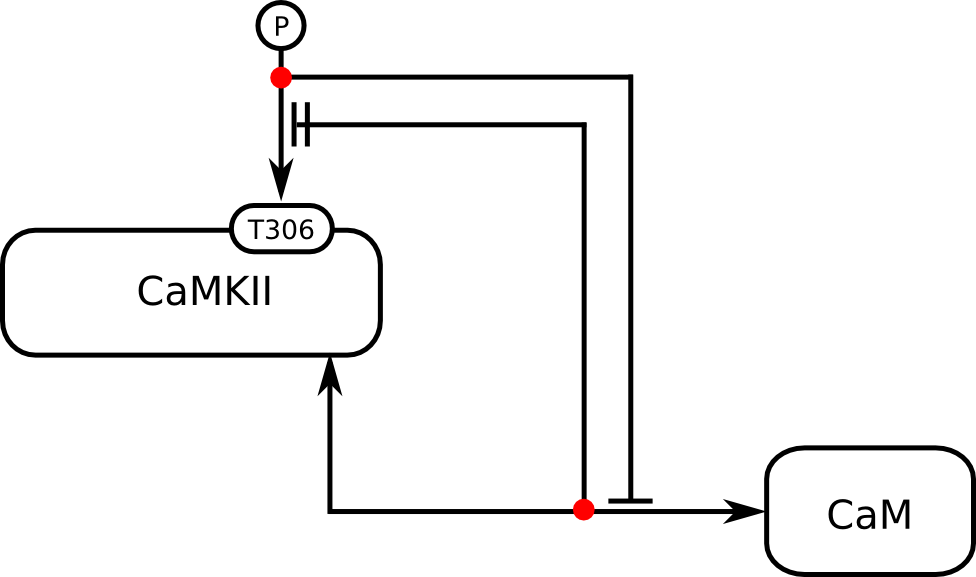
\includegraphics[scale = 0.5]{examples/ex-outcome}
  \caption{Examples of \glyph{outcomes}. The rightmost represents the fact that calmodulin effectively interacts (\sect{interaction}) with calcium/calmodulin kinase II. The leftmost represents the fact that the value phosphorylated is assigned (\sect{assignment}) to the variable representing threonin 306 of calcium/calmodulin kinase II.}
  \label{fig:ex-outcome}
\end{figure}

%\normalcolor
	
